\documentclass{article}[18pt]
\usepackage{../../../../format}
\lhead{A Level Maths - M2}

\usetikzlibrary{positioning} %Used for diagram at bottom


\begin{document}
\begin{center}
\underline{\huge M2 Cheat Sheet}
\end{center}
\section{Centres of mass}
\subsection{How to find the centre of mass of a system of particles of given position and mass}
\begin{tabularx}{\textwidth}{|X|X|X|X|X|}
\hline
Mass&&&&\\
\hline
Distance&&&&\\
\hline
\end{tabularx}
$$\bar{x}=\dfrac{\Sigma m_ix_i}{\Sigma m_i}$$
$$\bar{y}=\dfrac{\Sigma m_iy_i}{\Sigma m_i}$$
\subsection{How to locate centre of mass by appeal to symmetry}
In some cases, centre of mass may be balanced around a point due to symmetry, this will make calculations easier.
\subsection{How to find the centre of mass of a composite body}
In a body with many different shapes, put the masses into the table and the associated distances and treat as normal.\\
If all the composite shapes are the same, don't bother to find the true mass, set the mass of each shape to 1 and carry on.
\subsection{How to use the position of the centre of mass in problems involving the equilibrium of a rigid body}
When asked to the angle the vertical makes with a side when suspended about a point, draw the vertical from the point to the centre of mass, then use known distances to find the angle.\\
\\
In a more complicated question when you are given an angle, use trig to find the ratio between the two sides that are not the hypotenuse, then solve simultaneously to find what is needed
\section{Energy, work and power}
\subsection{How to calculate the work done by a force}
$$WD=FS$$
\subsection{How to calculate kinetic and gravitational potential energy}
$$KE=\frac{1}{2}mv^2$$
$$GPE=mgh$$
\subsection{The term mechanical energy and the work energy principle}
\textbf{The work energy principle} - The work done by all forces on a particle equals the change in kinetic energy of the particle\\
\textbf{Mechanical energy} - The sum of the kinetic and potential energy of an object
\subsection{How to apply the concept of power to the solution of problems}
$$P=Fv$$
\newpage
\section{Equilibrium of a rigid body}
$$\textrm{Moment}=\textrm{Force}\times\textrm{Perpendicular distance from the line of action of the force to the point}$$
\section{Momentum, restitution and impulse}
\subsection{What momentum is and how to calculate it}
$$\textrm{Momentum}=mv$$
Momentum is a vector quantity\\
Definition - The quantity of motion of a moving body
\subsection{Conservation of momentum}
In all collisions, momentum is conserved
$$m_1u_1+m_2u_2=m_1v_1+m_2v_2$$
\subsection{Coefficient of restitution}
$$e=\frac{SoS}{SoA}$$
If e=1, the collision is perfectly elastic\\
If e=0, the collision is perfectly inelastic
\subsection{Impulse}
$$\textrm{Impulse}=Ft=m(v-u)$$
\section{Projectiles}
$$v=u+at$$
$$s=ut+\frac{1}{2}at^2$$
$$s=\frac{u+v}{2}t$$
$$v^2=u^2+2as$$
$$s=vt-\frac{1}{2}at^2$$
\subsection{Forces on a projectile}
Assume:
\begin{itemize}
\item Only force acting is gravity
\item Projectile is a particle
\item Projectile is not powered
\item Air has no effect on the motion
\end{itemize}
There is no horizontal acceleration for the projectile
\subsection{Equation for path of a projectile (don't need to know, but might be useful)}
$$\ddot{x}=a=0$$
$$\dot{x}=v=v\cos\alpha$$
$$x=vt\cos\alpha$$
$$t=\frac{x}{v\cos\alpha}$$
\\
$$\ddot{y}=-g$$
$$\dot{y}=-gt+v\sin\alpha$$
$$y=-\frac{1}{2}gt^2+vt\sin\alpha$$
\\
$$y=-\frac{g}{2}\Bigg(\frac{x}{v\cos\alpha}\Bigg)^2+v\Bigg(\frac{x}{v\cos\alpha}\Bigg)\sin\alpha$$
$$y=x^2\Bigg(\frac{-g}{2v^2\cos^2\alpha}\Bigg)+x\Big(\tan\alpha\Big)$$
\section{Variable acceleration using differentiation and integration}
When using more than 1 dimension, consider each component separately \\
\begin{center}
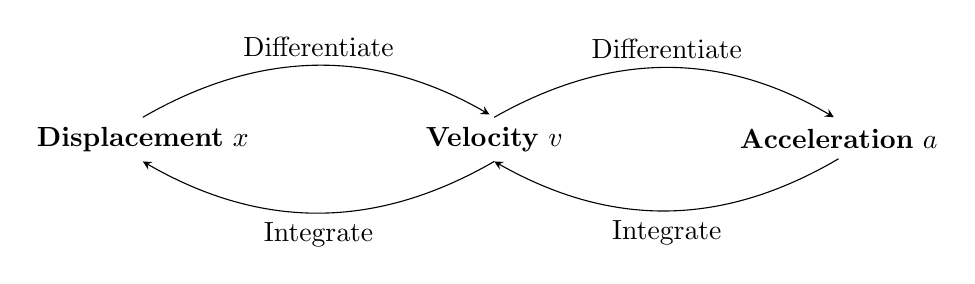
\begin{tikzpicture}
  \node (disp) {\textbf{Displacement} $x$};
  \node[right=2cm of disp] (vel) {\textbf{Velocity} $v$};
  \node[right=2cm of vel] (acc) {\textbf{Acceleration} $a$};
  \draw[-stealth,shorten >= 2pt] (disp.north) to[bend left] node[midway,above] {Differentiate} (vel.north);
  \draw[-stealth] (vel.south) to[bend left] node[midway,below] {Integrate} (disp.south);
  \draw[-stealth,shorten >= 2pt] (vel.north) to[bend left] node[midway,above] {Differentiate} (acc.north);
    \draw[-stealth] (acc.south) to[bend left] node[midway,below] {Integrate} (vel.south);
\end{tikzpicture}
\end{center}
\end{document}